\documentclass[letterpaper,10pt]{article}

\usepackage{enumitem}
\usepackage{titling}
\usepackage{listings,listings-rust}
\usepackage{url}
\usepackage{soul}
\usepackage{hyperref}
\usepackage{setspace}
\usepackage{subfig}
\usepackage{sectsty}
\usepackage{pdfpages}
\usepackage{colortbl}
\usepackage{multirow}
\usepackage{multicol}
\usepackage{relsize}
\usepackage{amsmath}
\usepackage{wasysym}
\usepackage{fancyvrb}
\usepackage[yyyymmdd]{datetime}
\usepackage{amsmath,amssymb,amsthm,graphicx,xspace}
\usepackage[titlenotnumbered,noend,noline]{algorithm2e}
\usepackage[compact]{titlesec}
\usepackage{XCharter}
\usepackage[T1]{fontenc}
\usepackage[scaled]{beramono}
\usepackage[normalem]{ulem}
\usepackage{booktabs}
\usepackage{tikz}
\usetikzlibrary{arrows.meta,automata,shapes,trees,matrix,chains,scopes,positioning,calc,decorations.pathreplacing}
\tikzstyle{block} = [rectangle, draw, fill=blue!20, 
    text width=2.5em, text centered, rounded corners, minimum height=2em]
\tikzstyle{bw} = [rectangle, draw, fill=blue!20, 
    text width=4em, text centered, rounded corners, minimum height=2em]

\definecolor{namerow}{cmyk}{.40,.40,.40,.40}
\definecolor{namecol}{cmyk}{.40,.40,.40,.40}
\renewcommand{\dateseparator}{-}

\let\LaTeXtitle\title
\renewcommand{\title}[1]{\LaTeXtitle{\textsf{#1}}}

\lstset{basicstyle=\footnotesize\ttfamily,breaklines=true}

\newcommand{\CPP}{C\nolinebreak\hspace{-.05em}\raisebox{.4ex}{\tiny\bf +}\nolinebreak\hspace{-.10em}\raisebox{.4ex}{\tiny\bf +}}
\def\CPP{{C\nolinebreak[4]\hspace{-.05em}\raisebox{.4ex}{\tiny\bf ++}}}

\newcommand{\handout}[5]{
  \noindent
  \begin{center}
  \framebox{
    \vbox{
      \hbox to 5.78in { {\bf ECE459: Programming for Performance } \hfill #2 }
      \vspace{4mm}
      \hbox to 5.78in { {\Large \hfill #4  \hfill} }
      \vspace{2mm}
      \hbox to 5.78in { {\em #3 \hfill \today} }
    }
  }
  \end{center}
  \vspace*{4mm}
}

\newcommand{\lecture}[3]{\handout{#1}{#2}{#3}{Lecture #1}}
\newcommand{\tuple}[1]{\ensuremath{\left\langle #1 \right\rangle}\xspace}

\addtolength{\oddsidemargin}{-1.000in}
\addtolength{\evensidemargin}{-0.500in}
\addtolength{\textwidth}{2.0in}
\addtolength{\topmargin}{-1.000in}
\addtolength{\textheight}{1.75in}
\addtolength{\parskip}{\baselineskip}
\setlength{\parindent}{0in}
\renewcommand{\baselinestretch}{1.5}
\newcommand{\term}{Winter 2021}

\singlespace


\begin{document}

\lecture{26 --- Profilers, Profiler Guided Optimization}{\term}{Patrick Lam \& Jeff Zarnett}

      \section*{Profilers}
Most profiling tools can gather more data than we've seen in the previous
topic. Your tools are typically aware of the whole
system, but may focus on one application, and may have both
per-process and system-wide modes. Frequently, though, you will find you can
use only the per-process mode if you're not a system administrator. That's not
super surprising, though, for security reasons. And for the same reason, in 
per-process mode you can usually see that the kernel was called, but no
details about what's going on inside. 

We'll discuss a couple more of these tools here, highlighting conceptual differences between these applications. They're all slightly different in how they work, but they get the job done.

\paragraph{Solaris Studio Performance Analyzer.} This 
tool\footnote{You can find a high-level description at
  \url{http://www.oracle.com/technetwork/server-storage/solarisstudio/documentation/oss-performance-tools-183986.pdf}}
supports {\tt gprof}-style profiling (``clock-based profiling'') as
well as kernel-level profiling through DTrace (described later). At
process level, it collects more process-level data than {\tt gprof},
including page fault times and wait times. It also can read CPU
performance counters (e.g. the number of executed floating point adds
and multiplies).  As a Sun application, it also works with Java
programs.

Since locks and concurrency are important, modern tools, including the
Studio Performance Analyzer, can track the amount of time spent
waiting for locks, as well as statistics about MPI message
passing. More on lock waits below, when we talk about WAIT.

\paragraph{VTune.} Intel and AMD both provide profiling
tools; Intel's VTune tool costs money, while AMD's CodeAnalyst tool is
free software.

Intel uses the term ``event-based sampling'' to refer to sampling 
which fires after a certain number of CPU events occur, and ``time-based
sampling'' to refer to the {\tt gprof}-style sampling (e.g. every 100ms).
VTune can also correlate the behaviour of the counters with other
system events (like disk workload). Both of these sampling modes
also include the behaviour of the operating system and I/O in their
counts.

VTune also supports an instrumentation-based profiling approach,
which measures time spent in each procedure (same type of
data as {\tt gprof}, but using a different collection scheme).

VTune will also tell you what it thinks the top problems with your
software are. However, if you want to understand what it's saying,
you do actually need to understand the architecture.

\paragraph{CodeAnalyst.} AMD also provides a profiling tool. Unlike Intel's tool, AMD's tool is
free software (the Linux version is released under the GPL), so that,
for instance, Mozilla suggests that people include CodeAnalyst
profiling data when reporting Firefox performance
problems~\footnote{\url{https://developer.mozilla.org/Profiling_with_AMD_CodeAnalyst}}.

CodeAnalyst is a system-wide profiler. It supports drilling down into
particular programs and libraries; the only disadvantage of being
system-wide is that the process you're interested in has to execute
often enough to show up in the profile. It also uses debug symbols to
provide meaningful names; these symbols are potentially supplied over
the Internet.

Like all profilers, it includes a sampling mode, which it calls ``Time-based
profiling'' (TBP). This mode works on all processors. The other modes are 
``Event-based profiling'' (EBP) and ``Instruction-based sampling'' (IBS);
these modes use hardware performance counters.

AMD's CodeAnalyst documentation points out that your sampling interval
needs to be sufficiently high to capture useful data, and that you need to 
take samples for enough time. The default sampling rate is once every
millisecond, and they suggest that programs should run for at least 15 seconds
to get meaningful data.

The EBP mode works like VTune's event-based sampling: after a certain
number of CPU events occur, the profiler records the system state.
That way, it knows where e.g. all the cache misses are occuring.
A caveat, though, is that EBP can't exactly identify the guilty statement,
because of ``skid'': in the presence of out-of-order execution, guilt
gets spread to the adjacent instructions.

To improve the accuracy of the profile information, CodeAnalyst uses
AMD hardware features to watch specific x86 instructions and ``ops'',
their associated backend instructions. This is the IBS mode\footnote{Available
on AMD processors as of the K10 family---typically manufactured in 2007+; see \url{http://developer.amd.com/assets/AMD_IBS_paper_EN.pdf}. Thanks to Jonathan Thomas for pointing this out.} of
CodeAnalyst.  AMD provides an
example\footnote{\url{http://developer.amd.com/cpu/CodeAnalyst/assets/ISPASS2010_IBS_CA_abstract.pdf}}
where IBS tracks down the exact instruction responsible for data
translation lookaside buffer (DTLB) misses, while EBP indicates four
potential guilty instructions.




\paragraph{DTrace.} 
DTrace~\cite{Cantrill:2004:DIP:1247415.1247417} is an instrumentation-based
system-wide profiling tool designed to be used on production
systems. It supports custom queries about system behaviour: when you
are debugging system performance, you can collect all sorts of data
about what the system is doing. The two primary design goals were in
support of use in production: 1) avoid overhead when not tracing and
2) guarantee safety (i.e. DTrace can never cause crashes).

DTrace runs on Solaris and some BSDs. There is a Linux port, which may be usable.
I'll try to install it on {\tt ece459-1}.

\paragraph{Probe effect.} ``Wait! Don't `instrumentation-based' 
and `production systems' not go together?'' For instance, Valgrind incurs a 100$\times$
slowdown. Ouch.

Nope! DTrace was designed to have zero overhead when inactive. It does
this by dynamically rewriting the code to insert instrumentation when
requested. So, if you want to instrument all calls to the {\tt open}
system call, then DTrace is going to replace the instruction at the
beginning of {\tt open} with an unconditional branch to the
instrumentation code, execute the profiling code, then return to your
code. Otherwise, the code runs exactly as if you weren't looking.

\paragraph{Safety.} As I've mentioned before, crashing a production
system is a big no-no. DTrace is therefore designed to never cause a
system crash. How? The instrumentation you write for DTrace 
must conform to fairly strict constraints.

\paragraph{DTrace system design.} The DTrace framework supports instrumentation
\emph{providers}, which make \emph{probes} (i.e.  instrumentation
points) available; and \emph{consumers}, which enable probes as
appropriate. Examples of probes include system calls, arbitrary kernel
functions, and locking actions. Typically, probes apply at function entry or exit points.
DTrace also supports typical
sampling-based profiling in the form of timer-based probes; that is,
it executes instrumentation every 100ms. This is tantamount to
sampling.

You can specify a DTrace clause using probes, predicates, and a set of
action statements. The action statements execute when the condition
specified by the probe holds and the predicate evaluates to true. D
programs consist of a sequence of clauses.

\paragraph{Example.} Here's an example of a DTrace query from~\cite{Cantrill:2004:DIP:1247415.1247417}.

{ \begin{verbatim}
    syscall::read:entry {
            self->t = timestamp;
    }

    syscall::read:return
    /self->t/ {
            printf("%d/%d spent %d nsecs in read\n"
                pid, tid, timestamp - self->t);
    }
    \end{verbatim}
}

The first clause instruments all entries to the system call {\tt read}
and sets a thread-local variable {\tt t} to the current time. The
second clause instruments returns from {\tt read} where the
thread-local variable {\tt t} is non-zero, calling {\tt printf} to print out
the relevant data.

The D (DTrace clause language) design ensures that clauses cannot loop indefinitely
(since they can't loop at all), nor can they execute unsafe code;
providers are responsible for providing safety guarantees. Probes
might be unsafe because they might interrupt the system at a critical
time. Or, action statements could perform illegal writes. DTrace won't 
execute unsafe code.

\paragraph{Workflow.} Both the USENIX article~\cite{Cantrill:2004:DIP:1247415.1247417} and the
ACM Queue article~\cite{300ps} referenced above contain example usages of DTrace.
In high-level terms: first identify a problem; then, use
standard system monitoring tools, plus custom DTrace queries,
to collect data about the problem (and resolve it).

\section*{WAIT}
Another approach which recently appeared in the research literature is
the WAIT tool out of IBM. Unfortunately, this tool is not free and not
generally available. Let's talk about it anyways.

Like DTrace, WAIT is suitable for use in production environments. It
uses hooks built into modern Java Virtual Machines (JVMs) to analyze
their idle time. It performs a sampling-based analysis of the
behaviour of the Java VM. Note that its samples are quite infrequent;
they suggest that taking samples once or twice a minute is enough.  At
each sample, WAIT records the state of each of the threads, which
includes its call stack and participation in system locks. This data
enables WAIT to compute (using expert rules) an abstract ``wait
state''.  The wait state indicates what the process is currently doing
or waiting on, e.g. ``disk'', ``GC'', ``network'', or ``blocked''.

\paragraph{Workflow.} You run your application, collect data (using a
script or manually), and upload the data to the server. The server provides
a report which you use to fix the performance problems.
The report indicates processor utilization (idle, your application, GC, 
etc); runnable threads; waiting threads (and why they are waiting); 
thread states; and a stack viewer.

The paper presents six case studies where WAIT helped solve performance
problems, including deadlocks, server underloads, memory leaks, database
bottlenecks, and excess filesystem activity.

\paragraph{Algorithmic profiling.} Coppa et al~\cite{coppa2014input} have proposed another profiling tool,
  {\tt aprof}.
  \url{https://code.google.com/p/aprof/}
{
  \begin{quote}
  aprof is a Valgrind tool for performance profiling designed to help developers discover hidden asymptotic inefficiencies in the code. From one or more runs of a program, aprof measures how the performance of individual routines scales as a function of the input size, yielding clues to its growth rate and to the "big-O" of the program.
  \end{quote}
  }

\paragraph*{Other Applications of Profiling.} 
Here's a short tangent. Many of the concepts that we've seen for code
also apply to web pages. Google's Page Speed
tool\footnote{\url{http://code.google.com/speed/page-speed/}}, in
conjunction with Firebug, helps profile web pages, and provides
suggestions on how to make your web pages faster. Note that Page Speed
includes improvements for the web page's design, e.g. not requiring
multiple DNS lookups; leveraging browser caching; or combining images;
as well as traditional profiling for the JavaScript on your pages.

I also mentioned earlier that I used the profiling tool for CUDA to find out what was wrong with my N-Body program. I ran the command \texttt{nvprof target/release/nbody-cuda}, and in addition to the regular program output I got the following, which showed that the time was going to the kernel and I wasn't losing a lot in overhead:

{\scriptsize
\begin{verbatim}
==20734== Profiling application: target/release/nbody-cuda
==20734== Profiling result:
            Type  Time(%)      Time     Calls       Avg       Min       Max  Name
 GPU activities:  100.00%  10.7599s         1  10.7599s  10.7599s  10.7599s  calculate_forces
                    0.00%  234.72us         2  117.36us  100.80us  133.92us  [CUDA memcpy HtoD]
                    0.00%  94.241us         1  94.241us  94.241us  94.241us  [CUDA memcpy DtoH]
      API calls:   97.48%  10.7599s         1  10.7599s  10.7599s  10.7599s  cuStreamSynchronize
                    1.92%  211.87ms         1  211.87ms  211.87ms  211.87ms  cuCtxCreate
                    0.54%  59.648ms         1  59.648ms  59.648ms  59.648ms  cuCtxDestroy
                    0.04%  4.8704ms         1  4.8704ms  4.8704ms  4.8704ms  cuModuleLoadData
                    0.00%  404.72us         2  202.36us  194.51us  210.21us  cuMemAlloc
                    0.00%  400.58us         2  200.29us  158.08us  242.50us  cuMemcpyHtoD
                    0.00%  299.30us         2  149.65us  121.42us  177.88us  cuMemFree
                    0.00%  243.86us         1  243.86us  243.86us  243.86us  cuMemcpyDtoH
                    0.00%  85.000us         1  85.000us  85.000us  85.000us  cuModuleUnload
                    0.00%  41.356us         1  41.356us  41.356us  41.356us  cuLaunchKernel
                    0.00%  18.483us         1  18.483us  18.483us  18.483us  cuStreamCreateWithPriority
                    0.00%  9.0780us         1  9.0780us  9.0780us  9.0780us  cuStreamDestroy
                    0.00%  2.2080us         2  1.1040us     215ns  1.9930us  cuDeviceGetCount
                    0.00%  1.4600us         1  1.4600us  1.4600us  1.4600us  cuModuleGetFunction
                    0.00%  1.1810us         2     590ns     214ns     967ns  cuDeviceGet
                    0.00%     929ns         3     309ns     230ns     469ns  cuDeviceGetAttribute
\end{verbatim}
}

Oh, and for comparison, here's the one where I make much better use of the GPU's capabilities (with better grid and block settings):

{\scriptsize
\begin{verbatim}
=22619== Profiling result:
            Type  Time(%)      Time     Calls       Avg       Min       Max  Name
 GPU activities:   99.92%  417.53ms         1  417.53ms  417.53ms  417.53ms  calculate_forces
                    0.06%  236.03us         2  118.02us  101.44us  134.59us  [CUDA memcpy HtoD]
                    0.02%  93.057us         1  93.057us  93.057us  93.057us  [CUDA memcpy DtoH]
      API calls:   52.09%  417.54ms         1  417.54ms  417.54ms  417.54ms  cuStreamSynchronize
                   26.70%  214.00ms         1  214.00ms  214.00ms  214.00ms  cuCtxCreate
                   13.63%  109.26ms         1  109.26ms  109.26ms  109.26ms  cuModuleLoadData
                    7.42%  59.502ms         1  59.502ms  59.502ms  59.502ms  cuCtxDestroy
                    0.05%  364.08us         2  182.04us  147.65us  216.42us  cuMemcpyHtoD
                    0.04%  306.48us         2  153.24us  134.10us  172.37us  cuMemAlloc
                    0.04%  285.73us         2  142.86us  122.90us  162.83us  cuMemFree
                    0.03%  246.37us         1  246.37us  246.37us  246.37us  cuMemcpyDtoH
                    0.01%  61.916us         1  61.916us  61.916us  61.916us  cuModuleUnload
                    0.00%  26.218us         1  26.218us  26.218us  26.218us  cuLaunchKernel
                    0.00%  15.902us         1  15.902us  15.902us  15.902us  cuStreamCreateWithPriority
                    0.00%  9.0760us         1  9.0760us  9.0760us  9.0760us  cuStreamDestroy
                    0.00%  1.6720us         2     836ns     203ns  1.4690us  cuDeviceGetCount
                    0.00%  1.0950us         1  1.0950us  1.0950us  1.0950us  cuModuleGetFunction
                    0.00%     888ns         3     296ns     222ns     442ns  cuDeviceGetAttribute
                    0.00%     712ns         2     356ns     212ns     500ns  cuDeviceGet
\end{verbatim}
}

\section*{Profiler Guided Optimization (POGO)}

In 2015 we were fortunate enough to have a guest lecture from someone at Microsoft actually in the room to give the guest lecture on the subject of Profile Guided Optimization (or POGO). In subsequent years, I was not able to convince him to fly in just for the lecture. Now there's a pandemic, so that's a big nope. Anyway, let's talk about the subject, which is by no means restricted to Rust.

The compiler does static analysis of the code you've written and makes its best guesses about what is likely to happen. The canonical example for this is branch prediction: there is an if-else block and the compiler will then guess about which is more likely and optimize for that version. Consider three examples, originally from~\cite{pogo} but replaced with some Rust equivalents:

\begin{lstlisting}[language=Rust]
fn which_branch(a: i32, b: i32) {
    if a < b {
        println!("Case one.");
    } else {
        println!("Case two.");
    }
}
\end{lstlisting}

Just looking at this, which is more likely, \texttt{a < b} or \texttt{a >= b}? Assuming there's no other information in the system the compiler can believe that one is more likely than the other, or having no real information, use a fallback rule. This works, but what if we are wrong? Suppose the compiler decides it is likely that \texttt{a} is the larger value and it optimizes for that version. However, it is only the case 5\% of the time, so most of the time the prediction is wrong. That's unpleasant. But the only way to know is to actually run the program.

\begin{multicols}{2}
\begin{lstlisting}[language=Rust]
trait Polite {
    fn greet(&self) -> String;
}

struct Kenobi {
    /* Stuff */
}
impl Polite for Kenobi {
    fn greet(&self) -> String {
        return String::from("Hello there!");
    }
}
\end{lstlisting}
\columnbreak
\begin{lstlisting}[language=Rust]
struct Grievous {
    /* Things */
}
impl Polite for Grievous {
    fn greet(&self) -> String {
        return String::from("General Kenobi.");
    }
}

fn devirtualization(thing: &Polite) {
    println!("{}", thing.greet());
}

\end{lstlisting}
\end{multicols}



There are similar questions raised for the other two examples. What is the ``normal'' type for some reference \texttt{thing}? It could be of either type \texttt{Kenobi} or \texttt{Grievous}. If we do not know, the compiler cannot do devirtualization (replace this virtual call with a real one). If there was exactly one type that implements the \texttt{Polite} trait we wouldn't have to guess. But are we much more likely to see \texttt{Kenobi} than \texttt{Grievous}?

\begin{lstlisting}[language=Rust]
fn match_thing(x: i32) -> i32 {
    match x {
        0..10 => 1,
        11..100 => 2,
        _ => 0
    }
}
\end{lstlisting}

 Same thing with \texttt{x}: what is its typical value? If we know that, it is our prediction. Actually, in a match block with many options, could we rank them in descending order of likelihood?

There exists a solution to this, and it is that we can give hints to the compiler, but that's a manual process. Automation is a good thing and this lecture is about that. These sorts of things already exist for Java! The Java HotSpot virtual machine will update its predictions on the fly. There are some initial predictions and if they turn out to be wrong, the Just In Time compiler will replace it with the other version. That's neat! I don't know for certain but I suspect the .NET runtime will do the same for something like C\#. But this is Rust and we don't have the runtime to reduce the overhead: the compiler runs and it does its job and that's it; the program is never updated with newer predictions if more data becomes known.

Solving this problem is the goal of POGO. It is taking the data from some actual runs of the program and using that to inform the predictions. This necessitates a multi-step compile: first compile the code, run it to collect data, then recompile the code using the data we collected. Let's expand on all three steps.

Step one is to generate an executable with instrumentation. Ask to compile with instrumentation enabled, which also says what directory to put it in: \texttt{-Cprofile-generate=/tmp/pgo-data}. The compiler inserts a bunch of probes into the generated code that are used to record data. Three types of probe are inserted: function entry probes, edge probes, and value probes.  A function entry probe, obviously, counts how many times a particular function is called. An edge probe is used to count the transitions (which tells us whether an if branch is taken or the else condition). Value probes are interesting; they are used to collect a histogram of values. Thus, we can have a small table that tells us the frequency of what is given in to a \texttt{match} statement. When this phase is complete, there is an instrumented executable and an empty database file where the training data goes~\cite{pogo}. 

Step two is training day: run the instrumented executable through real-world scenarios. Ideally you will spend the training time on the performance-critical sections. It does not have to be a single training run, of course, data can be collected from as many runs as desired. Keep in mind that the program will run a lot slower when there's the instrumentation present. 

Still, it is important to note that you are not trying to exercise every part of the program (this is not unit testing); instead it should be as close to real-world-usage as can be accomplished. In fact, trying to use every bell and whistle of the program is counterproductive; if the usage data does not match real world scenarios then  the compiler has been given the wrong information about what is important. Or you might end up teaching it that almost nothing is important... 

According to the docs about it\footnote{\url{https://doc.rust-lang.org/rustc/profile-guided-optimization.html}}, the output \texttt{.profraw} files require a little bit of processing before they're ready to go. When the program is running, the recording of data is done as quickly as possible with little regard for making it neat. Think of it like taking notes furiously during a lecture and then later revisiting them to organize them a bit. The tool for doing this is \texttt{llvm-profdata} and it will organize the data into a \texttt{.profdata} file. We can merge multiple runs as needed into a single file that will be used for input. 

Step three is a recompile. This time, in addition to the source files, the (merged) training data is fed into the compiler for a second compile, and this data is applied to (hypothetically) produce a better output executable than could be achieved by static analysis alone.


It is not necessary to do all three steps for every build. Old training data can be re-used until the code base has diverged significantly enough from the instrumented version. According to~\cite{pogo}, the recommended workflow is for one developer to perform these steps and check the training data into source control so that other developers can make use of it in their builds.

The Intel Developer Zone explains the process in a handy infographic\footnote{Source: \url{https://software.intel.com/en-us/node/522721}} :

\begin{center}
	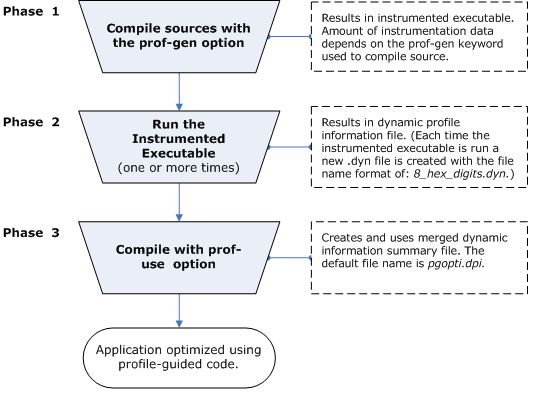
\includegraphics[width=0.5\textwidth]{images/pogo-workflow.jpg}
\end{center}



Or, here, a complete set of steps for actually running it if our program is all in \texttt{main.rs}, from the docs:

{\scriptsize
\begin{verbatim}
# STEP 1: Compile the binary with instrumentation
rustc -Cprofile-generate=/tmp/pgo-data -O ./main.rs

# STEP 2: Run the binary a few times, maybe with common sets of args.
#         Each run will create or update `.profraw` files in /tmp/pgo-data
./main mydata1.csv
./main mydata2.csv
./main mydata3.csv

# STEP 3: Merge and post-process all the `.profraw` files in /tmp/pgo-data
llvm-profdata merge -o ./merged.profdata /tmp/pgo-data

# STEP 4: Use the merged `.profdata` file during optimization. All `rustc`
#         flags have to be the same.
rustc -Cprofile-use=./merged.profdata -O ./main.rs
\end{verbatim}
}

What does it mean for the executable to be better? We have already looked at an example about how to predict branches. Predicting it correctly will be faster than predicting it incorrectly, but this is not the only thing.  The algorithms will aim for speed in the areas that are ``hot'' (performance critical and/or common scenarios). The algorithms will alternatively aim to minimize the size of code of areas that are ``cold'' (not heavily used). It is recommended in~\cite{pogo} that less than 5\% of methods should be compiled for speed.

It is possible that we can combine multiple training runs and we can manually give some suggestions of what scenarios are important. Obviously the more a scenario runs in the training data, the more important it will be, as far as the POGO optimization routine is concerned, but multiple runs can be merged with user assigned weightings.

\subsection*{Behind the Scenes}

In the optimize phase, the training data is used to do the following optimizations( which I will point out are based on C and \CPP programs and not necessarily Rust, but the principles should work because the Rust compiler's approach to this is based on that of LLVM/Clang)~\cite{pogo2}:

\begin{multicols}{2}
\begin{enumerate}
\item Full and partial inlining
\item Function layout
\item Speed and size decision
\item Basic block layout 
\item Code separation
\item Virtual call speculation
\item Switch expansion
\item Data separation
\item Loop unrolling
\end{enumerate}
\end{multicols}

For the most part we should be familiar with the techniques that are listed as being other compiler optimizations we have previously discussed. The new ones are (3) speed and size decision, which we have just covered; and items (4) and (5) which relate to how to pack the generated code in the binary.

According to~\cite{pogo2} the majority of the performance gains relate to the inlining decisions. These decisions are based on the call graph path profiling: the behaviour of function \texttt{foo} may be very different when calling it from \texttt{bar} than it is when calling it from function \texttt{baz}. Let's look at this call graph from~\cite{pogo2}:

\begin{center}
	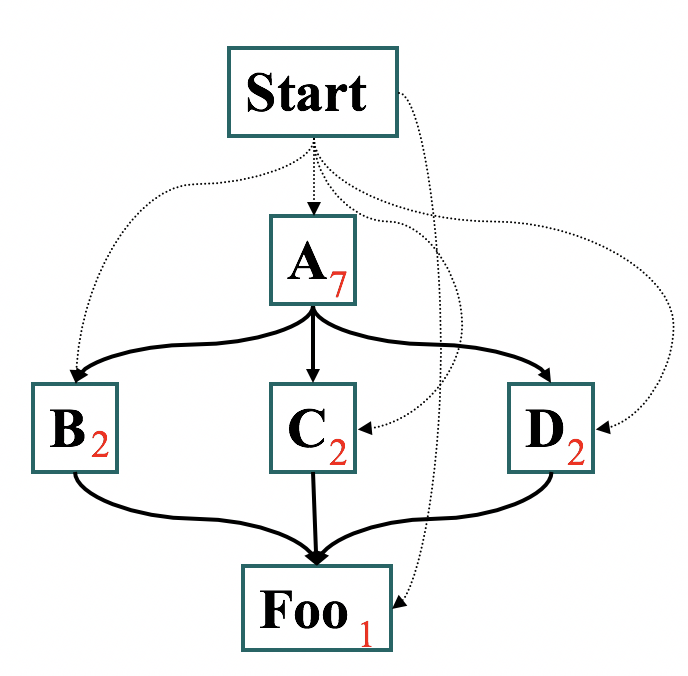
\includegraphics[width=0.25\textwidth]{images/callpaths.png}
\end{center}

Quick analysis of this code would have us find all the ways in which the functions might call each other. In total, there are 14 paths in this code, seven of which get us to function \texttt{Foo}. Consider another diagram showing the relationships between functions, in which the numbers on the edges represent the number of invocations~\cite{pogo2}:

\begin{center}
	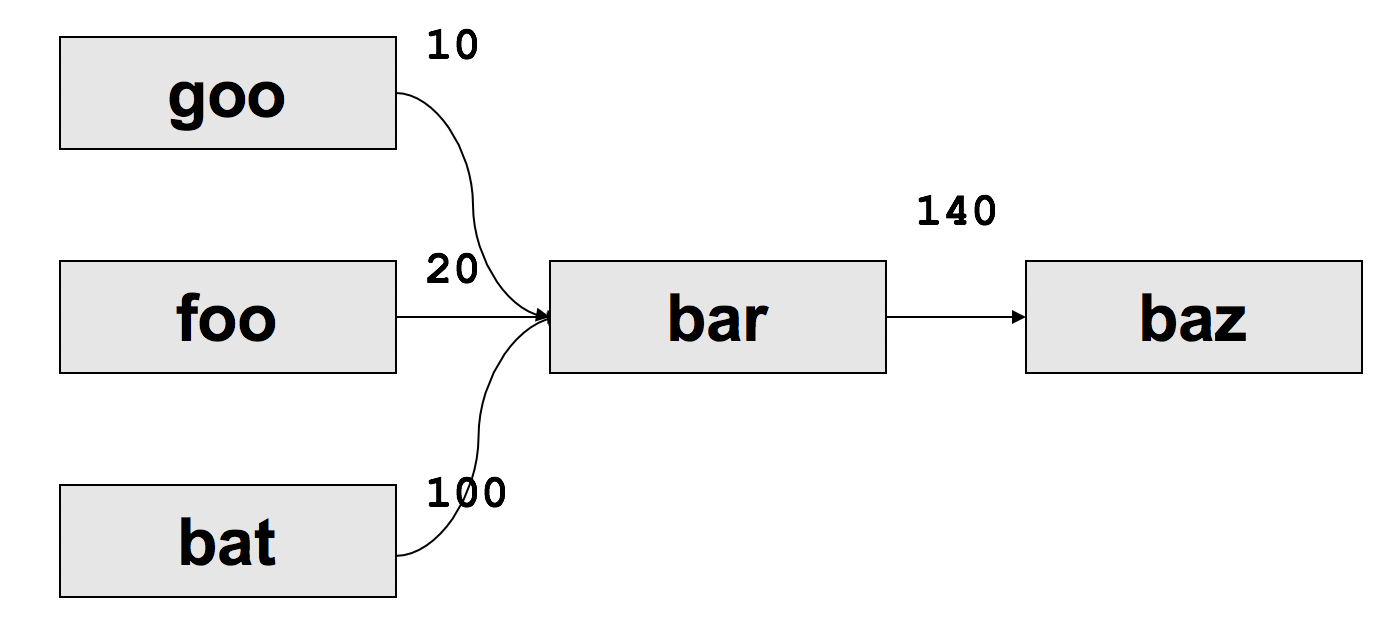
\includegraphics[width=0.4\textwidth]{images/callpaths2.png}
\end{center}

When considering what to do here, POGO takes the view like this~\cite{pogo2}:

\begin{center}
	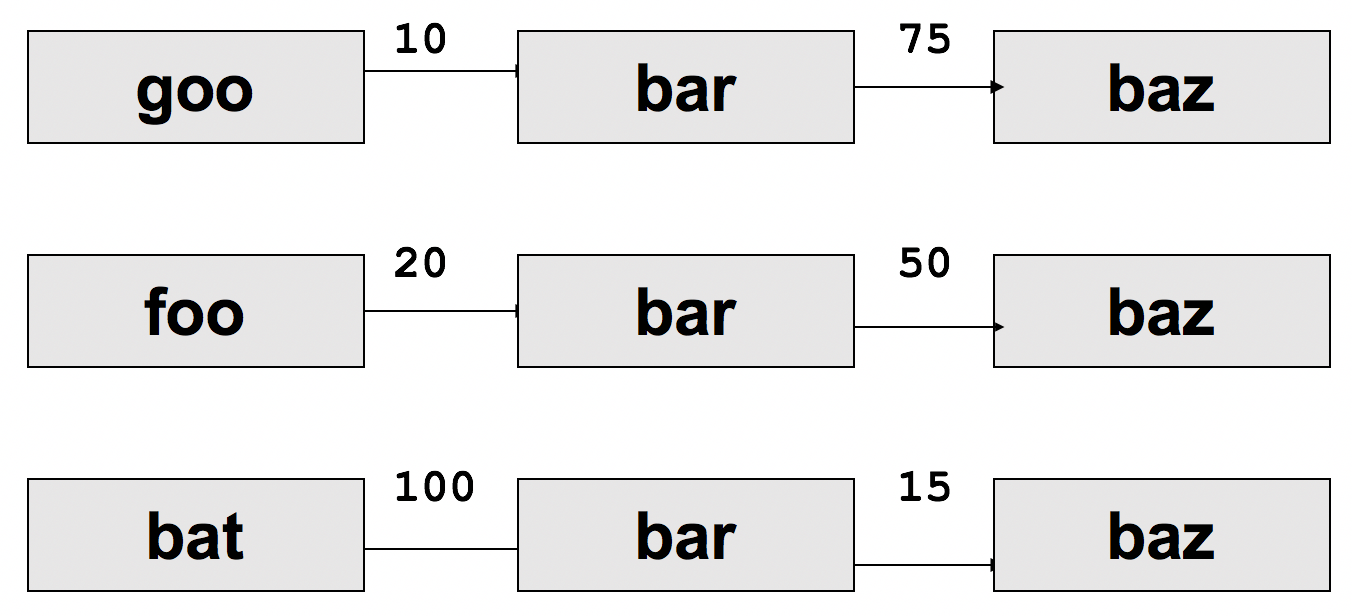
\includegraphics[width=0.4\textwidth]{images/callpaths3.png}
\end{center}

Each part of the call path is considered separately, remembering that we want to inline where it makes sense for speed, but otherwise leave it alone because of code size increases. Inlining \texttt{bar} into \texttt{bat} makes sense, but not inlining \texttt{bar} into \texttt{goo} (because that increases the code size without significant performance benefits). It also makes sense for \texttt{baz} to get inlined into \texttt{bar}. This is illustrated below~\cite{pogo2}:

\begin{center}
	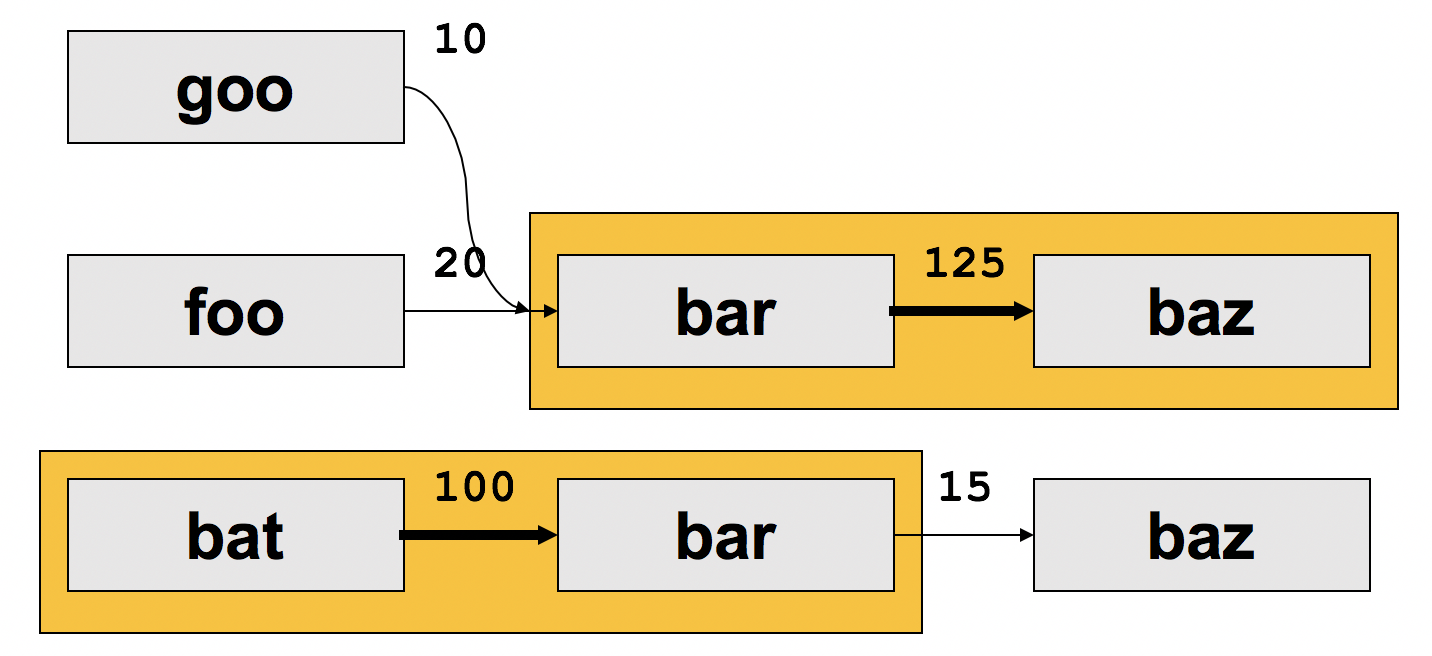
\includegraphics[width=0.4\textwidth]{images/callpaths4.png}
\end{center}

Packing the blocks is also done based on this call graph profiling. The most common cases will be put next to each other, and, where possible, subsequent steps are put next to each other. The more we can pack related code together, the fewer page faults we get by jumping to some other section, causing a cache miss... If the function being called is in the same page as the call, it has achieved ``page locality'' (and that is the goal!). This is represented visually~\cite{pogo2}:

\begin{center}
	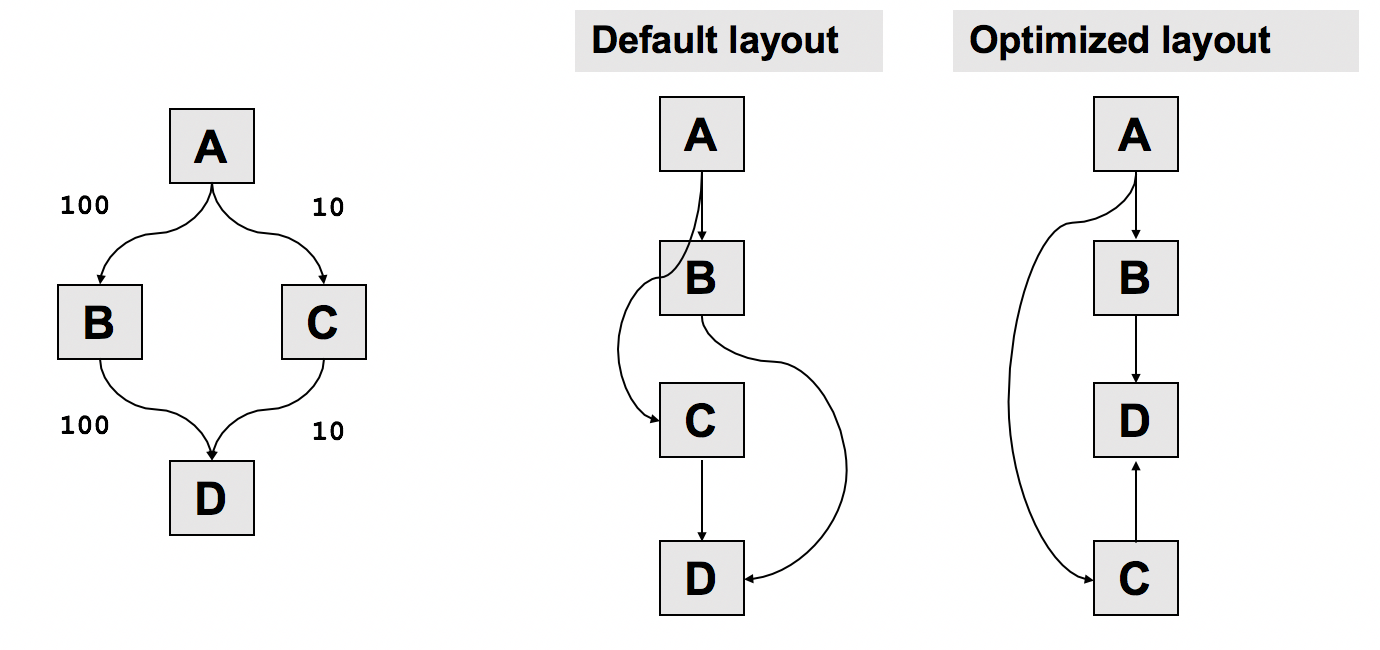
\includegraphics[width=0.6\textwidth]{images/blocklayout.png}
\end{center}

According to the author, the ``dead'' code goes in its own special block. I don't think they actually mean truly dead code, the kind that is compile-time determined to be unreachable, but instead they mean code that never gets invoked in any of the training runs.

So, to sum up, the training data is used to identify what branches are likely to be taken, inlines code where that is a performance increase, and tries to pack the binary code in such a way as to reduce cache misses/page faults. How well does it work?

\subsection*{Benchmark Results}

This table, condensed from~\cite{pogo2} summarizes the gains to be made. The application under test is a standard benchmark suite (Spec2K) (admittedly, C rather than Rust, but the goal is to see if the principle of POGO works and not just a specific implementation):

\begin{center}
\begin{tabular}{l|l|l|l|l|l}
	\textbf{Spec2k:} & \textbf{sjeng} & \textbf{gobmk} & \textbf{perl} & \textbf{povray} & \textbf{gcc}\\ \hline
	\textbf{App Size:} &  {Small} & {Medium} & {Medium} & {Medium} & {Large} \\ \hline
	\textbf{Inlined Edge Count} & 50\% & 53\% & 25\% & 79\% & 65\% \\ \hline
	\textbf{Page Locality} & 97\% & 75\% & 85\% & 98\% & 80\% \\ \hline
	\textbf{Speed Gain} & 8.5\% & 6.6\% & 14.9\% & 36.9\% & 7.9\% \\ 
\end{tabular}
\end{center}

There are more details in the source as to how many functions are used in a typical run and how many things were inlined and so on. But we get enough of an idea from the last row of how much we are speeding up the program, plus some information about why. We can speculate about how well the results in a synthetic benchmark translate to real-world application performance, but at least from this view it does seem to be a net gain.


\bibliographystyle{alphaurl}
\bibliography{459}


\end{document}
